
\documentclass[letterpaper,hide notes,xcolor={table,svgnames},pdftex]{beamer}
\def\showexamples{t}


%\usepackage[svgnames]{xcolor}

%% Demo talk
%\documentclass[letterpaper,notes=show]{beamer}

\usecolortheme{crane}
\setbeamertemplate{navigation symbols}{}

\usetheme{MyPittsburgh}
%\usetheme{Frankfurt}

%\usepackage{tipa}

\usepackage{hyperref}
\usepackage{graphicx,xspace}
\usepackage[normalem]{ulem}

\newcommand\SF[1]{$\bigstar$\footnote{SF: #1}}



\newcounter{tmpnumSlide}
\newcounter{tmpnumNote}

% old question code
%\newcommand\question[1]{{$\bigstar$ \small \onlySlide{2}{#1}}}
% \newcommand\nquestion[1]{\ifdefined \presentationonly \textcircled{?} \fi \note{\par{\Large \textbf{?}} #1}}
% \newcommand\nanswer[1]{\note{\par{\Large \textbf{A}} #1}}


 \newcommand\mnote[1]{%
   \addtocounter{tmpnumSlide}{1}
   \ifdefined\showcues {~\tiny\fbox{\arabic{tmpnumSlide}}}\fi
   \note{\setlength{\parskip}{1ex}\addtocounter{tmpnumNote}{1}\textbf{\Large \arabic{tmpnumNote}:} {#1\par}}}

\newcommand\mmnote[1]{\note{\setlength{\parskip}{1ex}#1\par}}

%\newcommand\mnote[2][]{\ifdefined\handoutwithnotes {~\tiny\fbox{#1}}\fi
% \note{\setlength{\parskip}{1ex}\textbf{\Large #1:} #2\par}}

%\newcommand\mnote[2][]{{\tiny\fbox{#1}} \note{\setlength{\parskip}{1ex}\textbf{\Large #1:} #2\par}}

\newcommand\mquestion[2]{{~\color{red}\fbox{?}}\note{\setlength{\parskip}{1ex}\par{\Large \textbf{?}} #1} \note{\setlength{\parskip}{1ex}\par{\Large \textbf{A}} #2\par}\ifdefined \presentationonly \pause \fi}

\newcommand\blackboard[1]{%
\ifdefined   \showblackboard
  {#1}
  \else {\begin{center} \fbox{\colorbox{blue!30}{%
         \begin{minipage}{.95\linewidth}%
           \hspace{\stretch{1}} Some space intentionally left blank; done at the blackboard.%
         \end{minipage}}}\end{center}}%
         \fi%
}



%\newcommand\q{\tikz \node[thick,color=black,shape=circle]{?};}
%\newcommand\q{\ifdefined \presentationonly \textcircled{?} \fi}

\usepackage{listings}
\lstset{%
  keywordstyle=\bfseries,
  aboveskip=15pt,
  belowskip=15pt,
  captionpos=b,
  identifierstyle=\ttfamily,
  escapeinside={(*@}{@*)},
  stringstyle=\ttfamiliy,
  frame=lines,
  numbers=left, basicstyle=\scriptsize, numberstyle=\tiny, stepnumber=0, numbersep=2pt}

\usepackage{siunitx}
\newcommand\sius[1]{\num[group-separator = {,}]{#1}\si{\micro\second}}
\newcommand\sims[1]{\num[group-separator = {,}]{#1}\si{\milli\second}}
\newcommand\sins[1]{\num[group-separator = {,}]{#1}\si{\nano\second}}
\sisetup{group-separator = {,}, group-digits = true}

%% -------------------- tikz --------------------
\usepackage{tikz}
\usetikzlibrary{positioning}
\usetikzlibrary{arrows,backgrounds,automata,decorations.shapes,decorations.pathmorphing,decorations.markings,decorations.text}

\tikzstyle{place}=[circle,draw=blue!50,fill=blue!20,thick, inner sep=0pt,minimum size=6mm]
\tikzstyle{transition}=[rectangle,draw=black!50,fill=black!20,thick, inner sep=0pt,minimum size=4mm]

\tikzstyle{block}=[rectangle,draw=black, thick, inner sep=5pt]
\tikzstyle{bullet}=[circle,draw=black, fill=black, thin, inner sep=2pt]

\tikzstyle{pre}=[<-,shorten <=1pt,>=stealth',semithick]
\tikzstyle{post}=[->,shorten >=1pt,>=stealth',semithick]
\tikzstyle{bi}=[<->,shorten >=1pt,shorten <=1pt, >=stealth',semithick]

\tikzstyle{mut}=[-,>=stealth',semithick]

\tikzstyle{treereset}=[dashed,->, shorten >=1pt,>=stealth',thin]

\usepackage{ifmtarg}
\usepackage{xifthen}
\makeatletter
% new counter to now which frame it is within the sequence
\newcounter{multiframecounter}
% initialize buffer for previously used frame title
\gdef\lastframetitle{\textit{undefined}}
% new environment for a multi-frame
\newenvironment{multiframe}[1][]{%
\ifthenelse{\isempty{#1}}{%
% if no frame title was set via optional parameter,
% only increase sequence counter by 1
\addtocounter{multiframecounter}{1}%
}{%
% new frame title has been provided, thus
% reset sequence counter to 1 and buffer frame title for later use
\setcounter{multiframecounter}{1}%
\gdef\lastframetitle{#1}%
}%
% start conventional frame environment and
% automatically set frame title followed by sequence counter
\begin{frame}%
\frametitle{\lastframetitle~{\normalfont(\arabic{multiframecounter})}}%
}{%
\end{frame}%
}
\makeatother

\makeatletter
\newdimen\tu@tmpa%
\newdimen\ydiffl%
\newdimen\xdiffl%
\newcommand\ydiff[2]{%
    \coordinate (tmpnamea) at (#1);%
    \coordinate (tmpnameb) at (#2);%
    \pgfextracty{\tu@tmpa}{\pgfpointanchor{tmpnamea}{center}}%
    \pgfextracty{\ydiffl}{\pgfpointanchor{tmpnameb}{center}}%
    \advance\ydiffl by -\tu@tmpa%
}
\newcommand\xdiff[2]{%
    \coordinate (tmpnamea) at (#1);%
    \coordinate (tmpnameb) at (#2);%
    \pgfextractx{\tu@tmpa}{\pgfpointanchor{tmpnamea}{center}}%
    \pgfextractx{\xdiffl}{\pgfpointanchor{tmpnameb}{center}}%
    \advance\xdiffl by -\tu@tmpa%
}
\makeatother
\newcommand{\copyrightbox}[3][r]{%
\begin{tikzpicture}%
\node[inner sep=0pt,minimum size=2em](ciimage){#2};
\usefont{OT1}{phv}{n}{n}\fontsize{4}{4}\selectfont
\ydiff{ciimage.south}{ciimage.north}
\xdiff{ciimage.west}{ciimage.east}
\ifthenelse{\equal{#1}{r}}{%
\node[inner sep=0pt,right=1ex of ciimage.south east,anchor=north west,rotate=90]%
{\raggedleft\color{black!50}\parbox{\the\ydiffl}{\raggedright{}#3}};%
}{%
\ifthenelse{\equal{#1}{l}}{%
\node[inner sep=0pt,right=1ex of ciimage.south west,anchor=south west,rotate=90]%
{\raggedleft\color{black!50}\parbox{\the\ydiffl}{\raggedright{}#3}};%
}{%
\node[inner sep=0pt,below=1ex of ciimage.south west,anchor=north west]%
{\raggedleft\color{black!50}\parbox{\the\xdiffl}{\raggedright{}#3}};%
}
}
\end{tikzpicture}
}


%% --------------------

%\usepackage[excludeor]{everyhook}
%\PushPreHook{par}{\setbox0=\lastbox\llap{MUH}}\box0}

%\vspace*{\stretch{1}

%\setbox0=\lastbox \llap{\textbullet\enskip}\box0}

\setlength{\parskip}{\fill}

\newcommand\noskips{\setlength{\parskip}{1ex}}
\newcommand\doskips{\setlength{\parskip}{\fill}}

\newcommand\xx{\par\vspace*{\stretch{1}}\par}
\newcommand\xxs{\par\vspace*{2ex}\par}
\newcommand\tuple[1]{\langle #1 \rangle}
\newcommand\code[1]{{\sf \footnotesize #1}}
\newcommand\ex[1]{\uline{Example:} \ifdefined \presentationonly \pause \fi
  \ifdefined\showexamples#1\xspace\else{\uline{\hspace*{2cm}}}\fi}

\newcommand\ceil[1]{\lceil #1 \rceil}


\AtBeginSection[]
{
   \begin{frame}
       \frametitle{Outline}
       \tableofcontents[currentsection]
   \end{frame}
}



\pgfdeclarelayer{edgelayer}
\pgfdeclarelayer{nodelayer}
\pgfsetlayers{edgelayer,nodelayer,main}

\tikzstyle{none}=[inner sep=0pt]
\tikzstyle{rn}=[circle,fill=Red,draw=Black,line width=0.8 pt]
\tikzstyle{gn}=[circle,fill=Lime,draw=Black,line width=0.8 pt]
\tikzstyle{yn}=[circle,fill=Yellow,draw=Black,line width=0.8 pt]
\tikzstyle{empty}=[circle,fill=White,draw=Black]
\tikzstyle{bw} = [rectangle, draw, fill=blue!20, 
    text width=4em, text centered, rounded corners, minimum height=2em]
    
    \newcommand{\CcNote}[1]{% longname
	This work is licensed under the \textit{Creative Commons #1 3.0 License}.%
}
\newcommand{\CcImageBy}[1]{%
	\includegraphics[scale=#1]{creative_commons/cc_by_30.pdf}%
}
\newcommand{\CcImageSa}[1]{%
	\includegraphics[scale=#1]{creative_commons/cc_sa_30.pdf}%
}
\newcommand{\CcImageNc}[1]{%
	\includegraphics[scale=#1]{creative_commons/cc_nc_30.pdf}%
}
\newcommand{\CcGroupBySa}[2]{% zoom, gap
	\CcImageBy{#1}\hspace*{#2}\CcImageNc{#1}\hspace*{#2}\CcImageSa{#1}%
}
\newcommand{\CcLongnameByNcSa}{Attribution-NonCommercial-ShareAlike}

\newenvironment{changemargin}[1]{% 
  \begin{list}{}{% 
    \setlength{\topsep}{0pt}% 
    \setlength{\leftmargin}{#1}% 
    \setlength{\rightmargin}{1em}
    \setlength{\listparindent}{\parindent}% 
    \setlength{\itemindent}{\parindent}% 
    \setlength{\parsep}{\parskip}% 
  }% 
  \item[]}{\end{list}} 




\title{Lecture 31 --- Android IV}

\author{Jeff Zarnett \\ \small \texttt{jzarnett@uwaterloo.ca}}
\institute{Department of Electrical and Computer Engineering \\[-1ex]
  University of Waterloo}
\date{\today}


\begin{document}

\begin{frame}
  \titlepage
\end{frame}

\part{Networking Basics}
\frame{\partpage}

\begin{frame}
\frametitle{Android Networking}

\begin{changemargin}{1cm}
One more lecture on advanced Android topics: networking.

Not necessary for the labs, but still examinable.

\end{changemargin}
\end{frame}

\begin{frame}[fragile]
\frametitle{Network Permissions}

\begin{changemargin}{1cm}
To access the network, permissions need to be assigned:
\end{changemargin}
{\scriptsize
\begin{verbatim}
<uses-permission android:name="android.permission.INTERNET" />
<uses-permission android:name="android.permission.ACCESS_NETWORK_STATE" />
\end{verbatim}
}
\end{frame}

\begin{frame}[fragile]
\frametitle{Network Availability}

\begin{changemargin}{1cm}
Good practice: check availability
{\scriptsize
\begin{verbatim}
ConnectivityManager connMgr = (ConnectivityManager) 
        getSystemService(Context.CONNECTIVITY_SERVICE);
    NetworkInfo networkInfo = connMgr.getActiveNetworkInfo();
    if (networkInfo != null && networkInfo.isConnected()) {
    ... // Do useful work
    }
\end{verbatim}
}
\end{changemargin}
\end{frame}

\begin{frame}
\frametitle{Networking}

\begin{changemargin}{1cm}
Networks are inherently unreliable.

They have unknown latency / bandwidth.

If we do network operations in the UI thread, we might get...

\end{changemargin}
\end{frame}

\begin{frame}
\frametitle{Not Responding}
\begin{changemargin}{3cm}
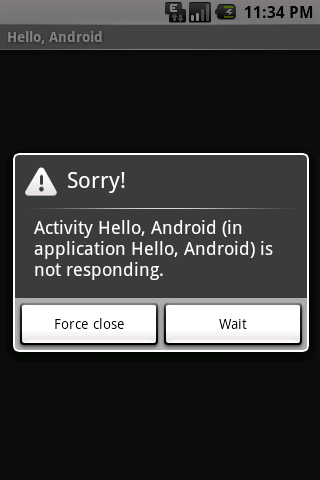
\includegraphics[width=0.45\textwidth]{images/anr.png}\\
(From linuxtopia.org)
\end{changemargin}
\end{frame}

\begin{frame}
\frametitle{Background Task}

\begin{changemargin}{1cm}
The not responding dialog doesn't appear because the program is hung.

It is doing a network operation and not redrawing the screen.

Solution: do work in the background with an \texttt{AsyncTask}.

\end{changemargin}
\end{frame}

\begin{frame}[fragile]
\frametitle{AsyncTask}


{\scriptsize
\begin{verbatim}
private class DownloadWebpageTask extends AsyncTask<String, Void, String> {
        @Override
        protected String doInBackground(String... urls) {
              
            // params comes from the execute() call: params[0] is the url.
            try {
                return downloadUrl(urls[0]);
            } catch (IOException e) {
                return "Unable to retrieve web page. URL may be invalid.";
            }
        }
        
        // onPostExecute displays the results of the AsyncTask.
        @Override
        protected void onPostExecute(String result) {
            textView.setText(result);
       }
    }
\end{verbatim}
}
\end{frame}

\begin{frame}
\frametitle{URL Downloader Task}

\begin{changemargin}{1cm}
This is a private class inside a \texttt{MainActivity} but it could be defined as an inner class.

Like a collection, such as \texttt{List}, the \texttt{AsyncTask} takes parameter types inside angle brackets for:\\
\quad \texttt{doInBackground}\\
\quad \texttt{onProgressUpdate}\\
\quad \texttt{onPostExecute}.

\end{changemargin}
\end{frame}

\begin{frame}
\frametitle{URL Downloader Task}

\begin{changemargin}{1cm}
AsyncTask execution goes through four stages:

\begin{enumerate}
\item \texttt{onPreExecute()}
\item \texttt{doInBackground(Params...)}
\item \texttt{onProgressUpdate(Progress...)}
\item \texttt{onPostExecute(Result)}
\end{enumerate}

\end{changemargin}
\end{frame}


\begin{frame}
\frametitle{Starting Tasks}

\begin{changemargin}{1cm}
To actually execute the Download Webpage task, use \texttt{new DownloadWebpageTask().execute(url);}

A task can be executed only once; to do something again, create another instance.

\end{changemargin}
\end{frame}

\begin{frame}
\frametitle{Cancelling Tasks}

\begin{changemargin}{1cm}
A task can be cancelled while it is running by calling \texttt{cancel(boolean)}.

This only makes \texttt{isCancelled()} return true.

The \texttt{doInBackground} method should check and see if the task has been cancelled.

Instead of \texttt{onPostExecute}, \texttt{onCancelled} runs.

\end{changemargin}
\end{frame}


\begin{frame}[fragile]
\frametitle{Excerpt from Networking Code}


{\scriptsize
\begin{verbatim}
HttpURLConnection conn = (HttpURLConnection) url.openConnection();
conn.setReadTimeout(10000 /* milliseconds */);
conn.setConnectTimeout(15000 /* milliseconds */);
conn.setRequestMethod("GET");
conn.setDoInput(true);
// Starts the query
conn.connect();
int response = conn.getResponseCode();
\end{verbatim}
}

Full code in the lecture notes.
\end{frame}

\begin{frame}
\frametitle{Using the Network}

\begin{changemargin}{1cm}

\texttt{HttpURLConnection} is the key to making the connection. 

Data can be of any type. 

Not necessary to know in advance the length of the data. 


\end{changemargin}
\end{frame}

\begin{frame}
\frametitle{HttpsURLConnection}

\begin{changemargin}{1cm}

Uses of this class follow a pattern:
\begin{enumerate}
\item Obtain a new \texttt{HttpURLConnection}.
\item Prepare the request. 
\item Optionally upload a request body.
\item Read the response.
\item Disconnect.
\end{enumerate}


\end{changemargin}
\end{frame}

\begin{frame}
\frametitle{HttpsURLConnection + SSL}

\begin{changemargin}{1cm}

Calling \texttt{openConnection()} on a URL with the "https" (HTTP with SSL, security) scheme will return an \texttt{HttpsURLConnection}. 

We are not going to cover this. 

For more detail and including things like posting content and authentication, take a look at the Android guidelines.

\end{changemargin}
\end{frame}

\part{Battery Life}
\frame{\partpage}

\begin{frame}
\frametitle{Battery Usage}

\begin{changemargin}{1cm}

Other than the screen, the next biggest user of battery is likely the wireless radio. 

The radio for a typical 3G divide has three states:

\begin{enumerate}
	\item Full Power
	\item Low Power
	\item Standby
\end{enumerate}


\end{changemargin}
\end{frame}

\begin{frame}
\frametitle{Radio State Transitions}

\begin{changemargin}{1cm}
Transition from one state to another is not instant. 
\end{changemargin}
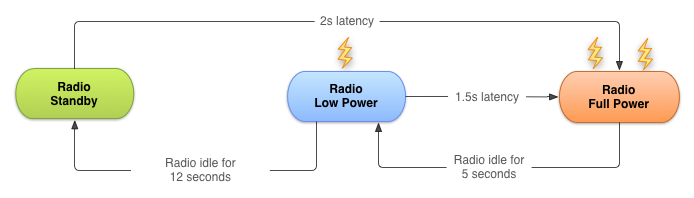
\includegraphics[width=\textwidth]{images/mobile_radio_state_machine.png}\\

\end{frame}

\begin{frame}
\frametitle{Battery Usage}

\begin{changemargin}{1cm}

Creating a new network connection puts the radio in the full power state.

A 1-second transfer is followed by:\\
\quad 5 seconds of ``tail time'' in the high power state\\
\quad 12 seconds in the low power state;

Then the radio returns to a standby state.

Total ``on'' time: 18 seconds.

\end{changemargin}
\end{frame}

\begin{frame}
\frametitle{Unbundled Data}

\begin{changemargin}{1cm}

Transfer data for 1 second every 18 seconds.

Radio never goes into standby $\rightarrow$ battery drain.

Out of every 60 seconds:\\
\quad 18 will be in the high power state;\\
\quad 42 will be in the low power state.

\end{changemargin}
\end{frame}

\begin{frame}
\frametitle{Bundled Data}

\begin{changemargin}{1cm}

Idea: bundle data (do transfers in bulk)

3 consecutive seconds of transfer means:\\
\quad 8 seconds in the high power state\\
\quad 12 seconds in the low power state.

40 seconds in the idle state!

\end{changemargin}
\end{frame}

\begin{frame}
\frametitle{Bundled vs. Unbundled}

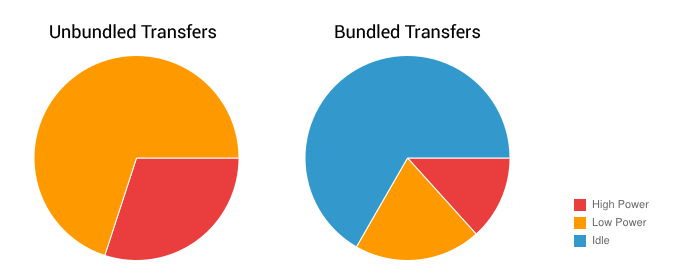
\includegraphics[width=\textwidth]{images/batteryusage.png}\\

\end{frame}

\part{Cloud Sync}
\frame{\partpage}

\begin{frame}
\frametitle{Cloud Sync}

\begin{changemargin}{1cm}

Sync your app with the cloud so data is not lost.

Even if the user reinstalls the app or changes device.

Google provides backup API for storing a small amount of data.

\end{changemargin}
\end{frame}

\begin{frame}[fragile]
\frametitle{Cloud Sync}

\begin{changemargin}{1cm}

Register for the service with Google.

Then implement Backup Agent:
{\scriptsize
\begin{verbatim}
<application android:label="MyApp"
             android:backupAgent="TheBackupAgent">
    ...
    <meta-data android:name="com.google.android.backup.api_key"
    android:value="ABcDe1FGHij2KlmN3oPQRs4TUvW5xYZ" />
    ...
</application>
\end{verbatim}
}

\end{changemargin}
\end{frame}

\begin{frame}[fragile]
\frametitle{Backup Agent}

{\scriptsize
\begin{verbatim}
 import android.app.backup.BackupAgentHelper;
 import android.app.backup.FileBackupHelper;


 public class TheBackupAgent extends BackupAgentHelper {
    // The name of the SharedPreferences file
    static final String HIGH_SCORES_FILENAME = "scores";

    // A key to uniquely identify the set of backup data
    static final String FILES_BACKUP_KEY = "myfiles";

    // Allocate a helper and add it to the backup agent
    @Override
    void onCreate() {
        FileBackupHelper helper = new FileBackupHelper(
              this, HIGH_SCORES_FILENAME);
        addHelper(FILES_BACKUP_KEY, helper);
    }
}
\end{verbatim}
}

\end{frame}

\begin{frame}
\frametitle{Cloud Sync}
\begin{changemargin}{1cm}
This \texttt{BackupAgentHelper} takes backups of the user's high scores file.

What if we used \texttt{SharedPreferences} instead of a file?
\end{changemargin}
\end{frame}


\begin{frame}[fragile]
\frametitle{Backup Agent}

{\scriptsize
\begin{verbatim}
 import android.app.backup.BackupAgentHelper;
 import android.app.backup.SharedPreferencesBackupHelper;

 public class TheBackupAgent extends BackupAgentHelper {
     static final String PREFS_DISPLAY = "displayprefs";
     static final String PREFS_SCORES = "highscores";

     // An arbitrary string used within the BackupAgentHelper implementation to
     // identify the SharedPreferencesBackupHelper's data.
     static final String MY_PREFS_BACKUP_KEY = "myprefs";

     // Simply allocate a helper and install it
     void onCreate() {
         SharedPreferencesBackupHelper helper =
                 new SharedPreferencesBackupHelper(
                     this, PREFS_DISPLAY, PREFS_SCORES);
         addHelper(MY_PREFS_BACKUP_KEY, helper);
     }
 }
\end{verbatim}
}

\end{frame}

\begin{frame}
\frametitle{Backup Semantics}
\begin{changemargin}{1cm}
To request a backup, create an instance of the \texttt{BackupManager}.

Call its \texttt{dataChanged()} method.

If you call \texttt{dataChanged()} more than once before the backup actually takes place, the backup will occur only once.

Restoring from backup happens automatically when the user reinstalls the application.

Can force it with \texttt{requestRestore()}. 
\end{changemargin}
\end{frame}


\begin{frame}
\frametitle{Sync Conflicts}
\begin{changemargin}{1cm}
It's possible that when you save data to the cloud you end up with conflicts. 

Some simple approaches to fixing it:

\begin{itemize}
\item Strategy 1: Newer is better.
\item Strategy 2: Value Judgement.
\item Strategy 3: Merge.
\end{itemize}
\end{changemargin}
\end{frame}


\begin{frame}
\frametitle{Sync Conflicts}
\begin{changemargin}{1cm}
These strategies work if the conflict and data are simple, but we might also have some more complex situations. 

If we are tracking something important like money, choosing the higher of the two values is an incorrect solution. 

Consider the following scenario where we just store the total:

\end{changemargin}
\end{frame}

\begin{frame}
\frametitle{Sync Conflicts}
\begin{changemargin}{1cm}

\begin{enumerate}
	\item Starting condition: the user has 0 coins on Device A, 0 on Device B.
	\item Player collects 10 coins on A.
	\item Player collects 15 coins on B.
	\item Device B saves.
	\item Device A saves - conflict detected.
	\item Conflict resolution: choose the largest of the two.
\end{enumerate}
Error occurred: player collected 25 coins but the value of 15 was chosen, so the user has ``lost'' 10 coins.

\end{changemargin}
\end{frame}

\begin{frame}
\frametitle{Sync Conflicts}
\begin{changemargin}{1cm}

Idea: send the delta instead of the values (e.g. ``+10'')

Android will send only the most recent update if network connectivity is not available. 

Imagine that the user collected 5 coins on A while on an airplane (network off).

Then in another session, collected another 5 coins. 

When the synchronization occurs, only the second update will be sent, so only 5 coins will be added to the user's total. 

Still incorrect.

\end{changemargin}
\end{frame}

\begin{frame}
\frametitle{Sync Conflicts}
\begin{changemargin}{1cm}

Solution: store sub-totals per device. 

Have a separate ``account'' for each device.

When the user collects 10 coins on device A, write it into a value for coins collected on A. 

Total: simply sum up the coins collected on A and B.


\end{changemargin}
\end{frame}



\end{document}
